\documentclass[11pt,utf8,notheorems,compress,t,aspectratio=169]{beamer}
\usepackage{etex}

\usepackage{pgfpages}
\usepackage[export]{adjustbox}

% Workaround for the issue described at
% https://tex.stackexchange.com/questions/164406/beamer-using-href-in-notes.
\newcommand{\fixedhref}[2]{\makebox[0pt][l]{\hspace*{\paperwidth}\href{#1}{#2}}\href{#1}{#2}}

\usepackage[english]{babel}

\usepackage{mathtools}
\usepackage{xspace}
\usepackage{booktabs}
\usepackage{stmaryrd}
\usepackage{amssymb}
\usepackage{manfnt}
\usepackage{array}
\usepackage{ragged2e}
\usepackage{multicol}
\usepackage{tabto}
\usepackage{xstring}
\usepackage{proof}
\usepackage{agda}
\usepackage[all]{xy}
\xyoption{rotate}
\usepackage{tikz}
\usetikzlibrary{calc,shapes,shapes.callouts,shapes.arrows,patterns,fit,backgrounds,decorations.pathmorphing,positioning,svg.path}
\hypersetup{colorlinks=true}
\usepackage[dvipsnames]{xcolor}
\usepackage{fontawesome5}

\DeclareFontFamily{U}{bbm}{}
\DeclareFontShape{U}{bbm}{m}{n}
   {  <5> <6> <7> <8> <9> <10> <12> gen * bbm
      <10.95> bbm10%
      <14.4>  bbm12%
      <17.28><20.74><24.88> bbm17}{}
\DeclareFontShape{U}{bbm}{m}{sl}
   {  <5> <6> <7> bbmsl8%
      <8> <9> <10> <12> gen * bbmsl
      <10.95> bbmsl10%
      <14.4> <17.28> <20.74> <24.88> bbmsl12}{}
\DeclareFontShape{U}{bbm}{bx}{n}
   {  <5> <6> <7> <8> <9> <10> <12> gen * bbmbx
      <10.95> bbmbx10%
      <14.4> <17.28> <20.74> <24.88> bbmbx12}{}
\DeclareFontShape{U}{bbm}{bx}{sl}
   {  <5> <6> <7> <8> <9> <10> <10.95> <12> <14.4> <17.28>%
      <20.74> <24.88> bbmbxsl10}{}
\DeclareFontShape{U}{bbm}{b}{n}
   {  <5> <6> <7> <8> <9> <10> <10.95> <12> <14.4> <17.28>%
      <20.74> <24.88> bbmb10}{}
\DeclareMathAlphabet{\mathbbm}{U}{bbm}{m}{n}
\SetMathAlphabet\mathbbm{bold}{U}{bbm}{bx}{n}

\usepackage{pifont}
\newcommand{\cmark}{\ding{51}}
\newcommand{\xmark}{\ding{55}}
\DeclareSymbolFont{extraup}{U}{zavm}{m}{n}
\DeclareMathSymbol{\varheart}{\mathalpha}{extraup}{86}

\graphicspath{{images/}}

\usepackage[protrusion=true,expansion=true]{microtype}

\setlength\parskip{\medskipamount}
\setlength\parindent{0pt}

\title{Modal operators for a constructive account of well quasi-orders}

\author{Ingo Blechschmidt}
\date{November 30th, 2024}

%\setbeameroption{show notes on second screen=bottom}
\newcommand{\jnote}[2]{\only<#1>{\note{\setlength\parskip{\medskipamount}\footnotesize\justifying#2\par}}}

%\useinnertheme[shadow=true]
\setbeamerfont{block title}{size={}}

\useinnertheme{rectangles}

\usecolortheme{orchid}
\usecolortheme{seahorse}
\definecolor{mypurple}{RGB}{253,73,34}
\definecolor{mypurpledark}{RGB}{100,0,150}
\setbeamercolor{structure}{fg=mypurple}
\setbeamercolor*{title}{bg=mypurple,fg=white}
\setbeamercolor*{titlelike}{bg=mypurple,fg=white}
\setbeamercolor{frame}{bg=black}

\usefonttheme{serif}
\usepackage[T1]{fontenc}
\usepackage{libertine}

% lifted from https://arxiv.org/abs/1506.08870
\DeclareFontFamily{U}{min}{}
\DeclareFontShape{U}{min}{m}{n}{<-> udmj30}{}
\newcommand\yon{\!\text{\usefont{U}{min}{m}{n}\symbol{'210}}\!}

\newcommand{\A}{\mathcal{A}}
\newcommand{\B}{\mathcal{B}}
\newcommand{\C}{\mathcal{C}}
\newcommand{\M}{\mathcal{M}}
\renewcommand{\AA}{\mathbb{A}}
\newcommand{\BB}{\mathbb{B}}
\newcommand{\pp}{\mathbbm{p}}
\newcommand{\MM}{\mathbb{M}}
\newcommand{\E}{\mathcal{E}}
\newcommand{\F}{\mathcal{F}}
\newcommand{\FF}{\mathbb{F}}
\newcommand{\G}{\mathcal{G}}
\newcommand{\J}{\mathcal{J}}
\newcommand{\GG}{\mathbb{G}}
\renewcommand{\O}{\mathcal{O}}
\newcommand{\K}{\mathcal{K}}
\newcommand{\NN}{\mathbb{N}}
\newcommand{\QQ}{\mathbb{Q}}
\newcommand{\RR}{\mathbb{R}}
\newcommand{\TT}{\mathbb{T}}
\newcommand{\PP}{\mathbb{P}}
\newcommand{\ZZ}{\mathbb{Z}}
\newcommand{\CC}{\mathbb{C}}
\renewcommand{\P}{\mathcal{P}}
\newcommand{\aaa}{\mathfrak{a}}
\newcommand{\bbb}{\mathfrak{b}}
\newcommand{\ccc}{\mathfrak{c}}
\newcommand{\ppp}{\mathfrak{p}}
\newcommand{\fff}{\mathfrak{f}}
\newcommand{\mmm}{\mathfrak{m}}
\newcommand{\defeq}{\vcentcolon=}
\newcommand{\defeqv}{\vcentcolon\equiv}
\newcommand{\Cov}{\mathrm{Cov}}
\renewcommand{\_}{\mathpunct{.}}
\newcommand{\?}{\,{:}\,}
\newcommand{\speak}[1]{\ulcorner\text{\textnormal{#1}}\urcorner}
\newcommand{\inv}{inv.\@}
\newcommand{\forces}{\vDash}
\newcommand{\ind}{\ensuremath{_\text{ind}}\xspace}
\newcommand{\sinf}{\ensuremath{_\infty}}
\newcommand{\impl}{\ensuremath{_\text{impl}}\xspace}
\newcommand{\formalized}{{\color{NavyBlue!75!White}{\raisebox{-0.5pt}{\scalebox{0.8}{\faCog}}}}}

\setbeamertemplate{blocks}[shadow=false]

\newenvironment{indentblock}{%
  \list{}{\leftmargin\leftmargin}%
  \item\relax
}{%
  \endlist
}

% Adapted from https://latex.org/forum/viewtopic.php?t=2251 (Stefan Kottwitz)
\newenvironment<>{hilblock}{
  \begin{center}
    \begin{minipage}{9.05cm}
      \setlength{\textwidth}{9.05cm}
      \begin{actionenv}#1
        \def\insertblocktitle{}
        \par
        \usebeamertemplate{block begin}}{
        \par
        \usebeamertemplate{block end}
      \end{actionenv}
    \end{minipage}
  \end{center}}

\newenvironment{changemargin}[2]{%
  \begin{list}{}{%
    \setlength{\topsep}{0pt}%
    \setlength{\leftmargin}{#1}%
    \setlength{\rightmargin}{#2}%
    \setlength{\listparindent}{\parindent}%
    \setlength{\itemindent}{\parindent}%
    \setlength{\parsep}{\parskip}%
  }%
  \item[]}{\end{list}}

\tikzset{
  invisible/.style={opacity=0,text opacity=0},
  visible on/.style={alt={#1{}{invisible}}},
  alt/.code args={<#1>#2#3}{%
    \alt<#1>{\pgfkeysalso{#2}}{\pgfkeysalso{#3}}}
}

% https://tex.stackexchange.com/questions/172336/drawing-roman-laurel-leaves-spqr-in-tikz
\tikzset{
  laurel-wreath/.pic = {
    \fill svg{M14.4-24.6c-1.5-1.5-2.6-3.3-3.1-5.3l-.4-1.7c-.2-1.1-.2-4.1 .2-5.7 .2-.9 .3-1.3 .5-1.3l1.4 1.1 2.5 2.4c2.7 2.5 5.2 6 5.8 8 .2 .6-.5 .3-2.2-.9-1.6-1.3-3.3-2.6-5-3.8l.1 1.4c.2 1.4 .5 2.7 1.1 4.6s.8 2.5 .5 2.5l-1.4-1.3zm69.6 1.1 .3-1.2c.8-2.3 1.3-4.8 1.6-7.3l-1.5 1.1c-1.3 .9-2.6 1.9-3.7 3-1.6 1.1-2 1.3-2.1 1 .7-1.8 1.6-3.4 2.8-4.9 1.3-1.7 6.5-6.8 7-6.8 .2 0 .3 .2 .3 .5l.3 1.6c.3 2.2 .2 5.7-.5 7.4-.8 1.9-1.6 3.1-3 4.7-1.1 1.1-1.4 1.3-1.5 .9z};
    \fill svg{M10-29.4c-.8-1.1-1.4-2.2-2-4.1l-.7-3.5c-.2-3 .2-4.4 1.4-8.3l.5-1.4c.2-1.3 .3-1.9 .6-1.9 .3-.2 .6 .3 .7 .8s.9 2.2 1.9 3.6c1.4 2.2 2.7 4.4 3.9 6.6l.9 2.7c0 .6 0 .6-.3 .6-.6 0-4.9-4.4-5.8-6l-.2-.6-.1 1.7-.3 2.8c-.3 2.7-.3 3.8 0 5.5 .6 2 .5 2.4-.5 1.5zm79.2 .3 .4-2.4c.2-1.3 .2-2.7-.1-4.9l-.3-2.8v-1.6l-.7 1c-.8 1.3-5 5.5-5.5 5.5s-.5-.3 .2-1.9c.5-1.7 1.4-3.3 3.3-6.5 2.4-3.6 2.7-3.9 2.8-4.7 .5-1.3 .5-1.4 .8-1.2 .3 0 .6 .8 .6 1.5l.7 2.4c.9 2.7 1.1 3.6 1.2 6 .2 3.1-.5 6-2 8.2-.8 1.3-1.3 1.7-1.4 1.5z};
    \fill svg{M5-40c-.4-3.2-.1-6.5 .9-9.6 .5-1.1 1.6-2.8 2.2-3.4l1.3-1.6 2-2.7 .2 .6c.1 1.3 .4 2.6 .9 3.8l.3 1c.8 1.7 1.1 2.7 1.6 5.3 .6 2.5 .6 4.6 .2 4.6-.3 0-.9-.8-1-1.1l-.5-.8c-1.4-2-3-5.2-2.9-6.5-.9 2.7-2 5.4-3.5 7.9l-.3 .8-.3 .8c0 .5-.6 1.6-.8 1.6l-.3-.7zm89.2 .2-.2-.5-.3-.9-1.1-2.7-1.1-2.4c-.6-1.4-1.2-2.8-1.6-4.2l-.3 .9c-.3 1.3-1.6 3.9-3 6-1.3 2-1.6 2-1.5 0s1.1-6.3 2.2-9c.8-1.7 1.1-3.1 .9-4.1-.2-1.1 .5-.8 2.2 1.8 3.3 4.4 3.8 5.4 4.4 7.8 .6 2.4 .5 7.7-.3 7.8l-.3-.5z};
    \fill svg{M13.9-50.1c-.5-1.9-.8-3.9-.9-5.8-.2-1.6-.1-3.3 .1-4.9-.3 .8-1.7 2.5-4.2 5.1l-3 4.9-.3 .1c-.3 0-.3-2.2 0-3.3 .8-3 1.4-4.6 2.5-6.1 .9-1.3 1.7-1.9 2.5-2.5 1.1-.6 2.7-1.9 3.5-2.7 .9-.9 1.9-1.4 2.2-1.4v1.1l-.3 6.6c0 6.8 .2 6.3-1 8.9-.5 1.1-.8 1.1-1.1 0zm70.8-.4c-.8-2.2-.8-2.5-.7-6.3-.1-2.7-.1-5.5-.2-8.2-.3-1.6-.3-1.9 .5-1.6l.6 .5c1.4 1.4 3 2.5 3.9 3.1 1.3 .9 1.9 1.6 2.7 2.6l.6 .7 .2 .4 .2 .3c.8 .9 2 4.9 2 6.9 .2 1.9-.2 1.9-.9 .5-.7-1.4-1.5-2.7-2.6-4-1.6-1.5-3-3.2-4.2-5 .4 3 .3 6-.5 9 0 .8-.5 2.2-.8 2.3-.2 0-.5-.3-.8-1.2z};
    \fill svg{M16.4-58.5l.2-1.5 .3-3.7c.2-2.8 .3-3.5 1.1-5.4l.7-1.3-.5 .4-1 .7c-.5 .4-1.1 .8-1.5 1.3l-.5 .3-1.9 1.6c-2.2 1.6-2.7 2-3.9 3.6-.5 .8-1.1 1.3-1.3 1.3-.5 0 0-2.4 1.1-4.7 1.5-3.4 4.3-6 7.7-7.4l1.3-.4 1.9-.4 2-.5c1.4 0 1.4 0 1 1.1-.5 .8-.8 2-1.1 4.2-.3 2.3-1.1 4.5-2.2 6.5l-.4 .6c-.6 1.1-1.3 2.1-2 3.2-.5 .6-.8 .8-1 .5zm66.3-.2c-.8-.9-2.8-4.4-3.5-6.1-.6-1.3-.9-2.5-1.1-3.5-.2-2.1-.7-4.1-1.5-6 0-.3 0-.3 1.2-.3l2.1 .5 1.9 .4 1.2 .4 .6 .1 1 .6c3 1.4 5.7 4.6 6.8 8.5l.7 2.6c-.2 .6-.5 .5-1.4-.7-2.2-2.7-4.8-5-7.7-6.9l-1.7-1.3 .6 1.3c.3 .6 .6 1.2 .8 1.9l.3 2.5 .3 3.9c.3 2.4 .2 2.8-.6};
    \fill svg{M21.6-66.1l.4-1.1 .9-3.2c.3-1.9 1.1-3.3 2.4-4.7l.4-.8-1.2 .2-2.2 .3c-2.7 .3-5.3 1.2-7.7 2.5-.6 .5-1.3 .6-1.3 .3 0-.5 .9-1.9 2-2.9 .8-.9 2-1.9 3.2-2.6l.9-.4 2.2-1c.3-.2 1.3-.3 3.2-.1 3 0 4.1 .2 6.3 .7l1.1 .4c.5 .2 .6 .6 .3 .6-.5 0-1.4 .9-1.9 1.7l-1.2 1.8c-1.7 2.8-2.2 3.5-4.6 5.9l-3 2.7-.2-.3zm53.9-2c-2.7-2.8-3.5-3.8-5.4-6.8-.9-1.6-1.4-2.4-1.9-2.5l-.8-.5c-.3 0-.2-.5 .4-.6l1.1-.4c1.9-.6 3-.8 5.6-.9l3.3 .2c2 .6 3.8 1.5 5.4 2.8 .3 0 1.9 1.6 2.5 2.4l.9 1.8c0 .3-.3 .2-1.9-.6-2.8-1.4-4.4-1.9-7.7-2.2l-2.2-.5c-.9-.2-.9-.2-.6 .2 .6 .5 1.7 2 2.1 2.8l.9 2.5c.3 1.5 .6 3 .9 4.6l-2.6-2.3z};
    \fill svg{M34.1-78.7c-3.4-1.3-6.9-2.1-10.6-2.5-.9 0-1.4 0-2.3 .3-2 .5-2 0 0-1.3l2.8-1.2c1.4-.5 1.9-.5 3.8-.6 3.8-.2 6.1 .3 9.3 1.7l3.6 1.1 2.2 .3c1.3 0 1.7 0 2.7-.3 1.1-.3 2.8-1.1 2.8-1.3l-1.3-.9c-1.9-1.4-3.1-2.7-3.1-3.2l.8-.6c.9-.3 1.3-.2 2 .8 .5 .8 1.1 1.4 2.9 2.7 .2 .3 .3 .2 1.1-.3 .9-.8 2.4-2 2.6-2.7 .5-.6 .9-.8 1.8-.5l.8 .6c0 .5-1.4 1.7-3.2 3.2l-1.3 .9c0 .2 1.7 .9 2.9 1.3 .9 .3 1.4 .3 2.7 .3l2.2-.3c1.7-.4 3.4-1 5-1.7 2-.8 4.4-1.3 7.7-1.1 2 .2 2.5 .2 3.8 .6 .9 .3 2.2 .8 2.8 1.2 2 1.1 2 1.6 .2 1.3-1.6-.3-1.9-.3-4.4 0-2.4 .3-4.7 .8-7 1.6l-1.5 .6c-2.9 .3-5.9 .2-8.8-.3-1.7-.3-3.6-.9-6-2.1l-1.1-.4-1.3 .6c-4.5 2.2-9.6 3-14.6 2.2zm-6.3-9.1c};
  }
}

\newcommand{\pointthis}[3]{%
  \tikz[remember picture,baseline]{
    \node[anchor=base,inner sep=0,outer sep=0] (#2) {#2};
    \node[visible on=#1,overlay,rectangle callout,rounded corners,callout relative pointer={(0.3cm,0.5cm)},fill=blue!20] at ($(#2.north)+(-0.1cm,-1.1cm)$) {#3};
  }%
}

\tikzset{
  invisible/.style={opacity=0,text opacity=0},
  visible on/.style={alt={#1{}{invisible}}},
  alt/.code args={<#1>#2#3}{%
    \alt<#1>{\pgfkeysalso{#2}}{\pgfkeysalso{#3}}}
}

\newcommand{\hcancel}[5]{%
  \tikz[baseline=(tocancel.base)]{
    \node[inner sep=0pt,outer sep=0pt] (tocancel) {#1};
    \draw[red!80, line width=0.4mm] ($(tocancel.south west)+(#2,#3)$) -- ($(tocancel.north east)+(#4,#5)$);
  }%
}

\newcommand{\explain}[7]{%
  \tikz[remember picture,baseline]{
    \node[anchor=base,inner sep=2pt,outer sep=0,fill=#3,rounded corners] (label) {#1};
    \node[anchor=north,visible on=<#2>,overlay,rectangle callout,rounded corners,callout
    relative pointer={(0.0cm,0.5cm)+(0.0cm,#6)},fill=#3] at ($(label.south)+(0,-0.3cm)+(#4,#5)$) {#7};
  }%
}

\newcommand{\explainstub}[2]{%
  \tikz[remember picture,baseline]{
    \node[anchor=base,inner sep=2pt,outer sep=0,fill=#2,rounded corners] (label) {#1};
  }%
}

\newcommand{\squiggly}[1]{%
  \tikz[remember picture,baseline]{
    \node[anchor=base,inner sep=0,outer sep=0] (label) {#1};
    \draw[thick,color=red!80,decoration={snake,amplitude=0.5pt,segment
    length=3pt},decorate] ($(label.south west) + (0,-2pt)$) -- ($(label.south east) + (0,-2pt)$);
  }%
}

% Adapted from https://latex.org/forum/viewtopic.php?t=2251 (Stefan Kottwitz)
\newenvironment<>{varblock}[2]{\begin{varblockextra}{#1}{#2}{}}{\end{varblockextra}}
\newenvironment<>{varblockextra}[3]{
  \begin{center}
    \begin{minipage}{#1}
      \begin{actionenv}#4
        {\centering \hil{#2}\par}
	\def\insertblocktitle{}%\centering #2}
        \def\varblockextraend{#3}
	\usebeamertemplate{block begin}}{
        \par
        \usebeamertemplate{block end}
        \varblockextraend
      \end{actionenv}
    \end{minipage}
  \end{center}}

\setbeamertemplate{headline}{}

\setbeamertemplate{frametitle}{%
  \leavevmode%
  \vskip-1.6em%
  \begin{beamercolorbox}[dp=1ex,center,wd=\paperwidth,ht=2.25ex]{title}%
    \vskip0.5em%
    \bf\insertframetitle
  \end{beamercolorbox}%

  \vskip-0.77em\hspace*{-2em}%
  \textcolor{mypurpledark}{\rule[0em]{1.1\paperwidth}{2.4pt}}

  \vskip-0.4em%
}

\setbeamertemplate{navigation symbols}{}

\newcounter{framenumberpreappendix}
\newcommand{\backupstart}{
  \setcounter{framenumberpreappendix}{\value{framenumber}}
}
\newcommand{\backupend}{
  \addtocounter{framenumberpreappendix}{-\value{framenumber}}
  \addtocounter{framenumber}{\value{framenumberpreappendix}}
}

\newcommand{\insertframeextra}{}
\setbeamertemplate{footline}{%
  \begin{beamercolorbox}[wd=\paperwidth,ht=2.25ex,dp=1ex,right,rightskip=1mm,leftskip=1mm]{}%
    % \inserttitle
    \hfill
    \insertframenumber\insertframeextra\,/\,\inserttotalframenumber
  \end{beamercolorbox}%
  \vskip0pt%
}

\newcommand{\hil}[1]{{\usebeamercolor[fg]{item}{\textbf{#1}}}}
\newcommand{\hill}[1]{{\usebeamercolor[fg]{item}{#1}}}
\newcommand{\bad}[1]{\textcolor{red!90}{\textnormal{#1}}}
\newcommand{\good}[1]{\textcolor{mypurple}{\textnormal{#1}}}

\newcommand{\bignumber}[1]{%
  \renewcommand{\insertenumlabel}{#1}\scalebox{1.2}{\!\usebeamertemplate{enumerate item}\!}
}
\newcommand{\normalnumber}[1]{%
  {\renewcommand{\insertenumlabel}{#1}\!\usebeamertemplate{enumerate item}\!}
}
\newcommand{\bigheart}{
\includegraphics{heart}}

\newcommand{\subhead}[1]{{\centering\textcolor{gray}{\hrulefill}\quad\textnormal{#1}\quad\textcolor{gray}{\hrulefill}\par}}

\newcommand{\badbox}[1]{\colorbox{red!30}{#1}}
\newcommand{\infobox}[1]{\colorbox{yellow!70}{\color{black}#1}}

% taken from JDH "The modal logic of arithmetic potentialism and the universal algorithm"
\DeclareMathOperator{\possible}{\text{\tikz[scale=.6ex/1cm,baseline=-.6ex,rotate=45,line width=.1ex]{\draw (-1,-1) rectangle (1,1);}}}
\DeclareMathOperator{\necessary}{\text{\tikz[scale=.6ex/1cm,baseline=-.6ex,line width=.1ex]{\draw (-1,-1) rectangle (1,1);}}}
\DeclareMathOperator{\xpossible}{\text{\tikz[scale=.6ex/1cm,baseline=-.6ex,rotate=45,line width=.1ex]{\draw (-1,-1) rectangle (1,1); \draw[very thin] (-.6,-.6) rectangle (.6,.6);}}}
\DeclareMathOperator{\xnecessary}{\text{\tikz[scale=.6ex/1cm,baseline=-.6ex,line width=.1ex]{\draw (-1,-1) rectangle (1,1); \draw[very thin] (-.6,-.6) rectangle (.6,.6);}}}

% Taken from Todd Lehman (CC-BY-SA) at https://tex.stackexchange.com/a/44920/32372

\newcommand{\setisprime}[1]{
  % Sets \isprime based on #1.
  \ifnum#1=1 \gdef\isprime{0} \else \gdef\isprime{1} \fi
  \foreach \sip in {2, 3,5,...,#1} {
    \pgfmathparse{\sip*\sip>#1? 1:0}
    \ifthenelse{\pgfmathresult=1}{
      % Early-out if \sip^2 > #1.
      \breakforeach
    }{
      % Otherwise test if \sip divides #1.
      \pgfmathparse{Mod(#1,\sip)==0? 1:0}
      \ifthenelse{\pgfmathresult=1}{
        \gdef\isprime{0}
        \breakforeach
      }{}
    }
  }
}

\newcommand{\setxy}[1]{
  % Sets \x and \y to loction of cell #1.
  \pgfmathtruncatemacro{\x}{Mod(#1-1,\cols)}
  \pgfmathtruncatemacro{\y}{(#1-1) / \cols}
  \pgfmathtruncatemacro{\y}{\cols - 1 - \y}
  \pgfmathparse{2.5*(\x+.5)}\let\x\pgfmathresult
  \pgfmathparse{2.5*(\y+.5)}\let\y\pgfmathresult
}

\newcommand{\numlabel}[2]{
  % Draws label #2 at cell #1.
  \setxy{\n}
  \node[fill=none, text=black] at (\x,\y) {#2};
}

\newcommand{\drawpolygon}[2]{
  % Draws polygon with #2 vertexes at cell #1.
  \setxy{#1}
  \ifthenelse{#2>1}{ % Polygon must have at least 2 sides.
    \ifthenelse{#2<30}{ % Draw polygon if it has a small number of sides.
      \filldraw (\x,\y) +(90:1)
      \foreach \drawi in {1,...,#2} {-- +(\drawi/#2*360+90:1)} -- cycle;
    }{ % Else approximate with circle.
      \filldraw (\x,\y) circle(1);
    }
  }{}
}

\newcommand{\setpolygoncolor}[1]{
  % Sets color based on #1.
  \gdef\polycolor{black}
  \ifnum#1=2\gdef\polycolor{black!50!white}\fi
  \ifnum#1=3\gdef\polycolor{yellow!95!red}\fi
  \ifnum#1=5\gdef\polycolor{yellow!0!red}\fi
  \ifnum#1=7\gdef\polycolor{blue!75!green}\fi
  \ifnum#1=11\gdef\polycolor{blue!70!red}\fi
  \ifnum#1=13\gdef\polycolor{blue!40!red}\fi
  \ifnum#1=17\gdef\polycolor{green!50!blue}\fi
  \ifnum#1=19\gdef\polycolor{green!80!black}\fi
  \ifnum#1=23\gdef\polycolor{green!50!red}\fi
  \ifnum#1=29\gdef\polycolor{yellow!50!black}\fi
  \ifnum#1=31\gdef\polycolor{orange!50!black}\fi
  \ifnum#1=37\gdef\polycolor{red!50!black}\fi
  \ifnum#1=41\gdef\polycolor{purple!50!black}\fi
  \ifnum#1=43\gdef\polycolor{blue!50!black}\fi
  \ifnum#1=47\gdef\polycolor{green!50!black}\fi
  \ifnum#1=53\gdef\polycolor{white!50!black}\fi
  \ifnum#1=59\gdef\polycolor{white!50!black}\fi
  \ifnum#1=61\gdef\polycolor{white!50!black}\fi
  \ifnum#1=67\gdef\polycolor{white!50!black}\fi
}

\newcommand{\sieve}[2]{
  \def\cols{#1}
  \def\rows{#2}
  \begin{tikzpicture}[scale=.5]
  \pgfmathtruncatemacro{\nmax}{\rows * \cols}

  \foreach \n in {1,...,\nmax} {
    \begin{scope}[fill=gray, fill opacity=.05,
                  draw=gray, draw opacity=.10,
                  line width=4]
      \drawpolygon{\n}{\n}
    \end{scope}
    \setisprime{\n}
    \ifthenelse{\isprime=1}{
      \numlabel{\n}{\bf\n}
    }{
      \def\startintensity{.33}
      \def\incrintensity{.10}
      \def\intensity{\startintensity}

      \def\m{\n}
      \pgfmathtruncatemacro{\i}{\m / 2}

      % Divide \m by \i until \m is extinguished.
      % Increment \i each time it does not divide into \m.
      \whiledo{\m>1}{
        \setisprime{\i}
        \pgfmathparse{Mod(\m,\i)==0? 1:0}
        \ifthenelse{\pgfmathresult=1\and\isprime=1}{
          \setpolygoncolor{\i}
          \begin{scope}[fill=\polycolor, fill opacity=\intensity,
                        draw=\polycolor!85!black, draw opacity=\intensity,
                        line width=\intensity*1.5]
            \drawpolygon{\n}{\i}
          \end{scope}
          \pgfmathtruncatemacro{\m}{\m / \i}
          \pgfmathparse{\intensity + \incrintensity}\let\intensity\pgfmathresult
        }{
          \pgfmathtruncatemacro{\i}{\i - 1}
          \def\intensity{\startintensity}
        }
      }
      \begin{scope}[text=black, text opacity=.5]
        \numlabel{\n}{\scriptsize\n}
      \end{scope}
    }
  }

  \end{tikzpicture}
}


\newcommand{\triang}{\hil{$\blacktriangleright$}}
\newcommand{\concat}{\mathbin{{+}\mspace{-8mu}{+}}}

\newcommand{\astikznode}[2]{\tikz[baseline,remember picture]{\node[anchor=base,inner sep=0,outer sep=0.1em] (#1) {#2};}}
\newcommand{\astikznodecircled}[3]{\tikz[baseline,remember picture]{\node[anchor=base,circle,draw=#2,thick,inner sep=0.05em,outer sep=0.05em] (#1) {#3};}}
\newcommand{\astikznodetransparentlycircled}[2]{\tikz[baseline,remember picture]{\node[anchor=base,circle,opacity=0,draw=white,text opacity=1,thick,inner sep=0.05em,outer sep=0.05em] (#1) {#2};}}

\setbeamersize{text margin left=1.60em,text margin right=1.60em}

\newlength\stextwidth
\newcommand\makesamewidth[3][c]{%
  \settowidth{\stextwidth}{#2}%
  \makebox[\stextwidth][#1]{#3}%
}

\newcommand{\dnote}[1]{%
  \begin{tabular}{@{}m{2em}@{}m{0.83\textwidth}@{}}%
    \textdbend &#1%
  \end{tabular}%
  \par
}

\newcommand{\genalpha}{\mbox{$\hspace{0.12em}\shortmid\hspace{-0.62em}\alpha$}}

\usepackage{newunicodechar}

\newunicodechar{∇}{\ensuremath{\nabla}}
\newunicodechar{λ}{\ensuremath{\lambda}}
\newunicodechar{σ}{\ensuremath{\sigma}}
\newunicodechar{τ}{\ensuremath{\tau}}
\newunicodechar{∷}{\ensuremath{::}}
\newunicodechar{⧺}{\ensuremath{\!\!\!}}
\newunicodechar{₁}{\ensuremath{_1}}
\newunicodechar{₂}{\ensuremath{_2}}
\newunicodechar{∈}{\ensuremath{\in}}
\newunicodechar{ℕ}{\ensuremath{\NN}}
\newunicodechar{↠}{\ensuremath{\twoheadrightarrow}}
\newunicodechar{ʳ}{\ensuremath{^r}}

\begin{document}

\addtocounter{framenumber}{-1}

\definecolor{mypurpleblack}{RGB}{30,0,50}
\setbeamercolor{structure}{fg=black}

{\usebackgroundtemplate{\begin{minipage}{\paperwidth}\centering\vspace*{-7em}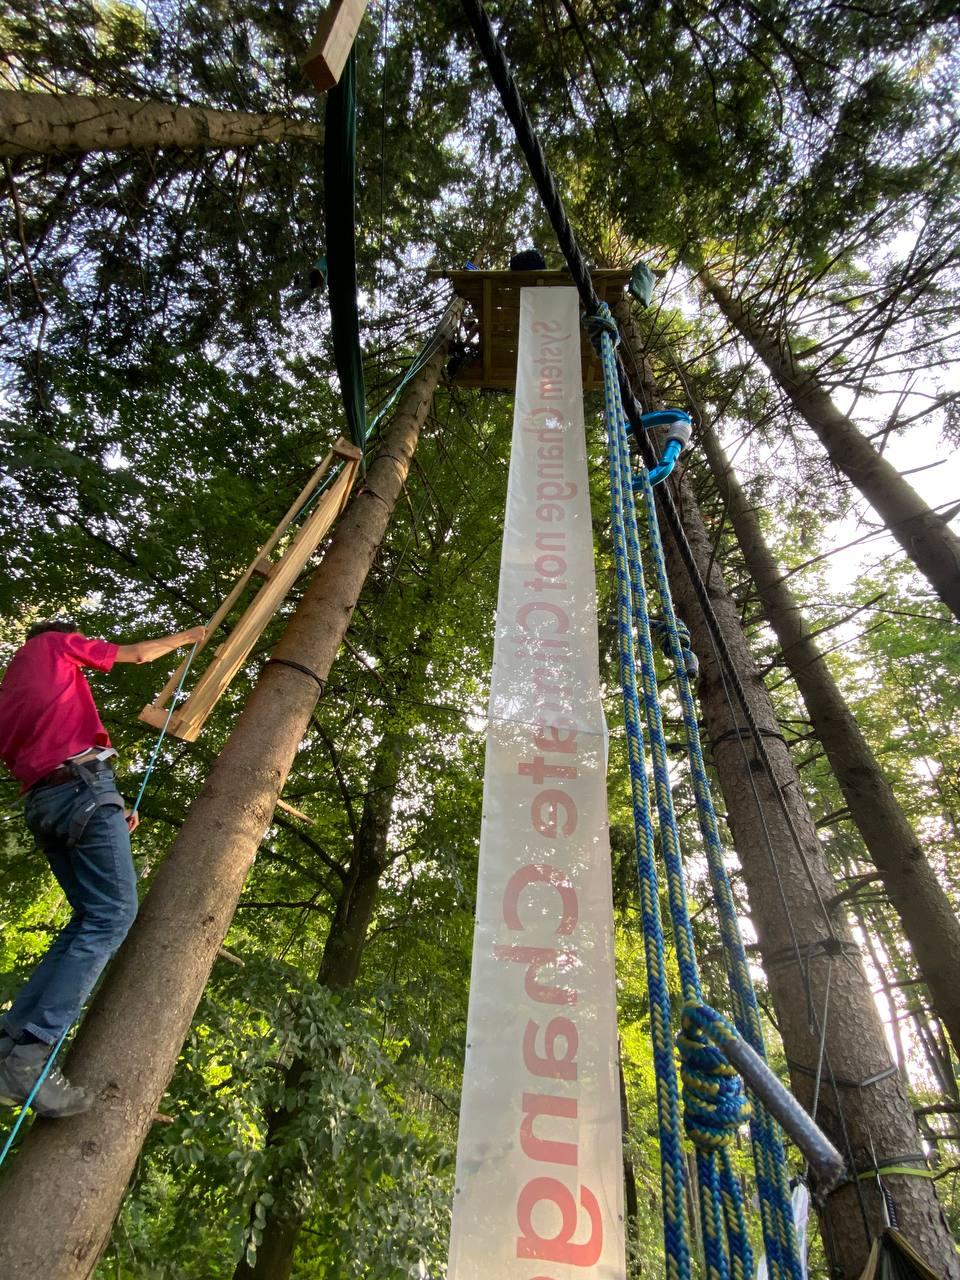
\includegraphics[width=\paperwidth]{forest2}\end{minipage}}
\begin{frame}[c]
  \centering
  \color{white}

  \bigskip
  \bigskip
  \bigskip
  \bigskip
  \bigskip
  \bigskip
  \bigskip
  \bigskip
  \bigskip

  \scriptsize

  \setbeamercolor{block body}{bg=black!100}
  \begin{minipage}{0.52\textwidth}
    \begin{block}{}
      \centering\normalsize\color{white}
      \hil{\color{white}Towards topological type theory for decrypting
      transfinite methods in classical~mathematics} \\[-0.4em]
      \
    \end{block}
  \end{minipage}

  \bigskip
  \bigskip
  \bigskip
  \bigskip
  \bf
  \colorbox{black}{\begin{minipage}{0.2\textwidth}
    \centering
    TYPES 2025 \\
    June 9th, 2025
  \end{minipage}}
  \bigskip

  \colorbox{black}{\begin{minipage}{0.2\textwidth}
    \centering
    Ingo Blechschmidt \\
    University of Antwerp
  \end{minipage}}
\end{frame}}

\definecolor{mypurple}{RGB}{150,0,255}
\setbeamercolor{structure}{fg=mypurple}

{\usebackgroundtemplate{\begin{minipage}{\paperwidth}\vspace*{1.7em}
\includegraphics[height=\paperheight]{sea-of-clouds-1}\end{minipage}}
\begin{frame}{A case study in Hilbert's program}
  \textbf{Def.} Let~$(X,{\leq})$ be a quasi-order.
  \vspace*{-0.3em}
  \begin{itemize}
    \item A sequence~$\alpha : \NN \to X$ is \hil{good} iff
    there merely exist~$i < j$ with~$\alpha\,i \leq \alpha\,j$.
    \item The quasi-order~$X$ is \hil{well\only<4->{\sinf}} iff every sequence~$\NN \to X$ is good.
  \end{itemize}
  \pause
  \vspace*{-1.3em}

  \begin{columns}[t]
    \begin{column}{0.46\textwidth}
      \begin{block}{Natural numbers\phantom{y}}
        \textbf{Prop.} $(\NN, {\leq})$ is well\only<4->{\sinf}. \formalized
        \smallskip

        \emph{Proof.} Let~$\alpha : \NN \to \NN$. By~\badbox{\textsc{lem}}, there is a
        \bad{minimum}~$\alpha\,i$.
        Set~$j \defeq i + 1$. \qed

        \hfill\color{gray}offensive?
      \end{block}
      \only<2-6>{
        \vspace*{-2em}
        \[ \astikznodetransparentlycircled{xm}{7}\!,
        \quad \astikznodetransparentlycircled{x0}{4}\!,
        \quad \astikznodecircled{t1}{mypurple}{3}\!,
        \quad \astikznodetransparentlycircled{x1}{1}\!,
        \quad \astikznodecircled{t2}{mypurple}{8}\!,
        \quad \astikznodetransparentlycircled{x2}{2}\!,
        \quad \ldots \]
      {\centering\begin{tikzpicture}[remember picture,overlay]
        \node[draw=mypurple, circle, thick, inner sep=0.1em] (t3) {\scriptsize$\leq$};
        \path[draw=mypurple,thick]
          (t1)
          to [out=-90, in=180] (t3)
          to [out=0, in=-90] (t2);
      \end{tikzpicture}\par}}
    \end{column}

    \pause

    \begin{column}{0.50\textwidth}
      \begin{block}{Key stability results}
        \justifying
        \only<1-5>{Assuming~\badbox{\textsc{lem}}
        and~\badbox{\textsc{dc}}}\only<6->{\good{Constructively}}, \ldots

        \hil{Dickson:} \tabto{1.7cm} If~$X$ and~$Y$ are well\only<4-5>{\sinf}\only<6->{\ind}, so is~$X \times Y$. \\
        \hil{Higman:}  \tabto{1.7cm} If~$X$ is well\only<4-5>{\sinf}\only<6->{\ind}, so is~$\mathrm{List}\,X$. \\
        \hil{Kruskal:} \tabto{1.7cm} If~$X$ is well\only<4-5>{\sinf}\only<6->{\ind}, so is~$\mathrm{Tree}\,X$.
      \end{block}
    \end{column}
  \end{columns}
  \pause
  \pause
  \pause
  \pause

  \textbf{Def.} A quasi-order~$X$ is \hil{well\ind} iff~$G\,[\,]$, where $G$ is
  the following inductively defined predicate on \hil{finite lists}.~\formalized{}
  (In presence of \bad{bar induction}, $\text{well}\ind \Leftrightarrow
  \text{well}\sinf$.)
  \[
    \small
    \infer{\mathsf{now}\,p : G\,\sigma}{p : \mathsf{Good}\,\sigma}
    \qquad
    \infer{\mathsf{later}\,f : G\,\sigma}{f : (x : X) \to G\,(\sigma ::^r x)}
  \]
  \vspace*{-1.3em}

  \only<8>{
    \begin{columns}[c]
      \begin{column}{0.01\textwidth}
	
\includegraphics[height=2.4em]{question-mark}
      \end{column}
      \begin{column}{0.9\textwidth}
      Is there a procedure for reinterpreting \hil{classical proofs}
      regarding well\sinf{} as \newline \hil{blueprints for constructive proofs} regarding well\ind?
      \end{column}
    \end{columns}
  }

  \only<9>{
    \vspace*{-0.0em}
    \hil{Central insight:} A quasi-order $X$ is well\ind iff $\hil{$\necessary$}\,\forall\alpha : \NN \to
    X\_ \exists i < j\_ \alpha\,i \leq \alpha\,j$.
  }
\end{frame}}

\begin{frame}{Missing functions in the type of all functions?}
  \begin{columns}[t]
    \begin{column}{0.57\textwidth}
      \begin{block}{Behold: A transfinite tool \ldots\phantom{g}}
        \justifying
        \textbf{Lemma.} \badbox{\textsc{lem}} Let~$X$ be well\sinf.
        Let~$\alpha : \NN \to X$. Then there is an increasing
        subsequence~$\alpha\,i_0 \leq \alpha\,i_1 \leq \cdots$.
      \end{block}

      \small
      \emph{Proof.}
      \begin{changemargin}{-0.8em}{0em}\begin{enumerate}\justifying
      \item The type
      $I \defeq \sum_{i \? \NN} \neg\sum_{j \? \NN} i < j \times \alpha\,i \leq
      \alpha\,j$
      is not in bijection with~$\NN$, as else the~$I$-extracted subsequence
      of~$\alpha$ would not be good.\smallskip
      \item By~\badbox{\textsc{lem}}, the type~$I$ is finite.\smallskip
      \item Any index~$i_0$ larger than all the indices in~$I$ is a suitable
      starting point for an increasing subsequence. \qed
      %  \item Let $\mathsf{Sad}\,i \defeq
      %  \neg \mathsf{Happy}\,i$ be the proposition
      %  expressing that~$i$ does not appear as the first component
      %  of a good pair, where
      %  $\mathsf{Happy}\,i \defeq \sum_{j \? \NN} i < j \times \alpha\,i \leq
      %  \alpha\,j$.
      %  \item If~$\mathsf{Sad}$ is anonymously dense in~$\NN$, i.e. $\forall a
      %  \? \NN\_ \neg\neg\exists b\?\NN\_ b \geq a \times \mathsf{Sad}\,b$, then
      %  \badbox{\textsc{lem}} and \badbox{\textsc{dc}} provide us with a
      %  subsequence~$\alpha\,k_0 \leq \alpha\,k_1 \leq \ldots$
      %  with~$\mathsf{Sad}\,k_0, \mathsf{Sad}\,k_1, \ldots$. This is a contradiction to wellness.
      %  \item
      %  Hence there is~\bad{not~not} an index~$a \? \NN$ such that~$\mathsf{Sad}$ is
      %  strictly bounded by~$a$; hence every index~$b \geq a$ does~\bad{not not} have
      %  a partner: $\forall b\geq a\_ \neg\neg\exists c>b\_
      %  \alpha\,b \leq \alpha\,c$. Thus~\bad{\textsc{lem}} and \bad{\textsc{dc}}
      %  provide us with the desired subsequence. \qed
      \end{enumerate}\end{changemargin}
    \end{column}

    \begin{column}{0.43\textwidth}
      \begin{block}{\ldots{} implying a concrete consequence}
        \textbf{Cor.} \badbox{\textsc{lem}}
        Let~$X$ and~$Y$ be well\sinf. Then~$X \times Y$ is
        well\sinf.\phantom{g}
      \end{block}

      \small
      \emph{Proof.}
      \begin{changemargin}{-0.8em}{0em}\begin{enumerate}\justifying
      \item Let a sequence~$\gamma : \NN \to X \times Y$ be
      given. Write~$\gamma\,k = (\alpha\,k,\beta\,k)$.\smallskip
      \item By the lemma, there is an
      increasing subsequence~$\alpha\,i_0 \leq \alpha\,i_1 \leq \cdots$.\smallskip
      \item Because~$Y$
      is well, there are indices~$n < m$ such that~$\beta\,i_n \leq
      \beta\,i_m$.\smallskip
      \item As
      also~$\alpha\,i_n \leq \alpha\,i_m$, the sequence~$\gamma$ is good. \qed
      \end{enumerate}\end{changemargin}
    \end{column}
  \end{columns}

  \dnote{\emph{We cannot trust~\bad{\textsc{lem}}-provided sequences to be
  available in the type~$\NN \to X$. Similarly with~\bad{\textsc{dc}}.}}
\end{frame}

{\usebackgroundtemplate{\begin{minipage}{\paperwidth}\vspace*{0.29cm}\hspace*{-1cm}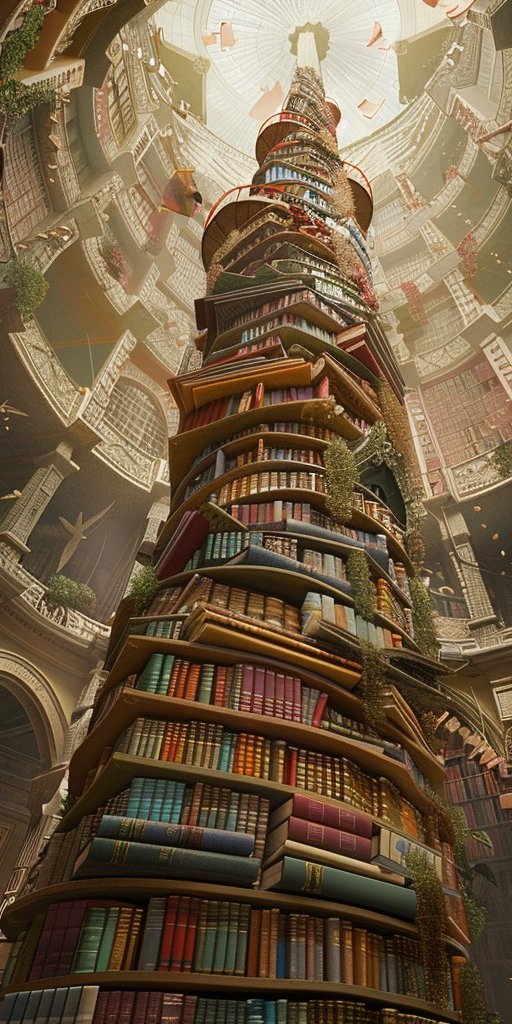
\includegraphics[height=\paperheight]{tower-cropped}\end{minipage}}
\begin{frame}{Where do many cherished inductive definitions come from?}
  \begin{changemargin}{8.0em}{-0.5em}
    In mathematics, we routinely enlarge structures:
    \begin{itemize}
      \small
      \item Pass from~$\mathbb{Q}$ to~$\mathbb{R}$, to embrace irrationals.
      \item Pass from~$\mathbb{R}$ to~$\mathbb{C}$, to obtain $\sqrt{-1}$.
      \item Pass from~$\mathbb{C}$ to~$\mathbb{C}[X]$, to obtain a ``generic number''.
    \end{itemize}

    In set and type theory, we can also enlarge \hil{the mathematical universe}:
    \begin{itemize}
      \small
      \item Force a \hil{generic sequence} $\NN \to X$. \formalized
      \item Force a \hil{generic enumeration} $\NN \twoheadrightarrow X$
            (even if $X$ is uncountable). \formalized
      \item Force a \hil{generic prime ideal} of a given ring. \formalized
    \end{itemize}
    \pause

    Central observations of the multiversal yoga:
    \begin{itemize}
      \small
      \item A quasi-order~$X$ is well\ind iff the generic sequence~$\NN \to X$
      is good. \formalized
      \item A relation is well-founded iff for the generic descending chain,
      $\bot$. \formalized
      \item A ring element is nilpotent iff it is contained in the generic
      prime ideal. \formalized
    \end{itemize}
    \pause

    The mystery of nongeometric sequents:
    \begin{itemize}
    \small
      \item The generic ring is a field.
      \item \ \\[-1.2em]\mbox{For the generic surjection $f : \NN \twoheadrightarrow \RR$,
      $\neg\neg \exists n \? \NN\_ f(n) = \pi \wedge f(n+1) = e$. \formalized}
    \end{itemize}
  \end{changemargin}
\end{frame}}

{\usebackgroundtemplate{\begin{minipage}{\paperwidth}\vspace*{4.95cm}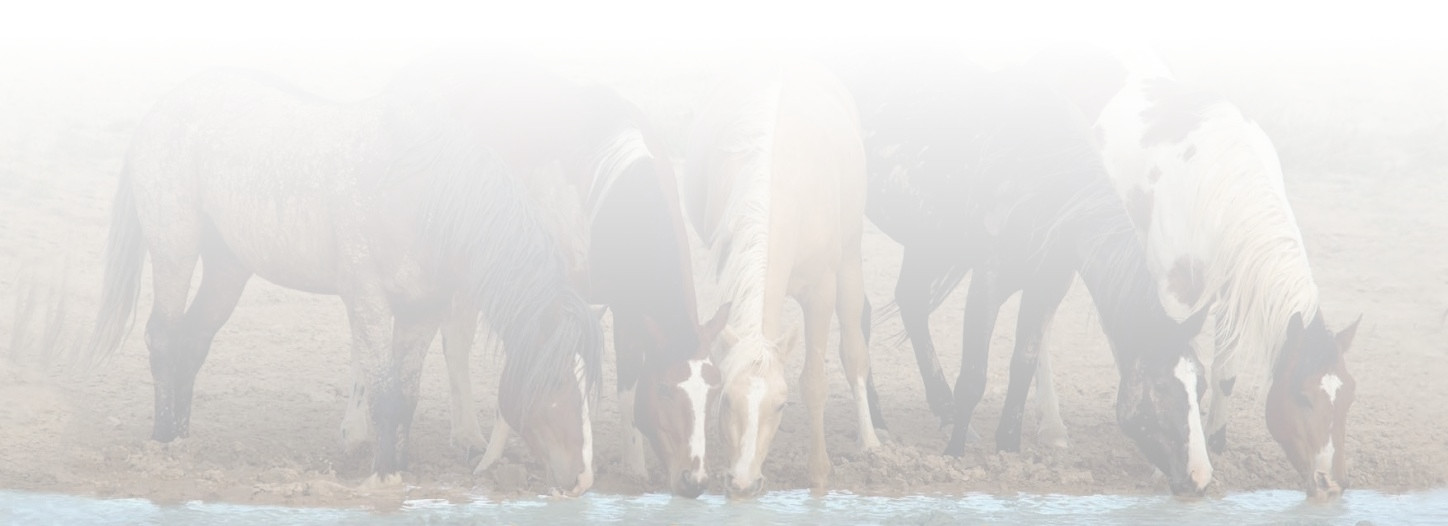
\includegraphics[width=\paperwidth]{topos-horses-lighter}\end{minipage}}
\begin{frame}{A modal language for harnessing the multiverse}
  \textbf{Def.} A statement~$\varphi$ holds \ldots
  \vspace*{-0.3em}
  \begin{itemize}
    \small
    \item \hil{everywhere} \tabto{2.05cm}($\necessary\varphi$)\tabto{2.98cm}
    iff it holds \hil{in every topos}
    (over the current base).
    \item \hil{somewhere} \tabto{2.05cm}($\possible\varphi$)\tabto{2.98cm} iff
    it holds \hil{in some positive topos}.
    \item \hil{proximally} \tabto{2.05cm}($\xpossible\varphi$)\tabto{2.98cm}
    iff it holds \hil{in some positive overt topos}.
  \end{itemize}

  We then have:
  \begin{enumerate}
    \item $\mathsf{Well}\ind(X,{\le}) \Longleftrightarrow
    \necessary\mathsf{Well}\sinf(X,{\le})$. \formalized
    \item $(\possible\varphi) \Longleftrightarrow \varphi$,
    if $\varphi$ is a geometric implication (``$\forall\ldots\forall (\%
    \Rightarrow \%)$'', with no~$\forall$ nor~$\Rightarrow$
    in~$\%$).~\formalized
    \item $(\xpossible\varphi) \Longleftrightarrow \varphi$,
    if~$\varphi$ is a bounded first-order statement. \formalized
    \item For every inhabited type~$X$, $\xpossible\necessary
    \mathsf{Countable}(X)$, where~$\mathsf{Countable}(X) \defeqv (\exists f : \NN
    \to X\_ \mathsf{Surjective}(f))$. \formalized

    So being countable is a \hil{button}.
    \item $\possible \badbox{\textsc{lem}}$.
    (Baby Barr / Friedman's trick / nontrivial exit continuation)

    In fact, \badbox{\textsc{lem}} is a \hil{switch}:
    $\necessary\bigl((\possible\badbox{\textsc{lem}}) \wedge
    (\possible\neg\badbox{\textsc{lem}})\bigr)$

    \item $\badbox{\textsc{zorn}} \Rightarrow
    \necessary\possible\badbox{\textsc{ac}}$. (Great Barr)
  \end{enumerate}
\end{frame}}

\begin{frame}{The plain combinatorics of toposes}
  \begin{enumerate}\justifying
    \item Realize a generic gadget as some kind of limit of \hil{approximations}
    from the base universe. For the generic function $f_0 : \NN \to X$:

    \AgdaHide{
      \begin{code}
open import Data.List
open import Agda.Primitive using (Set)

Prop = Set
postulate
  X : Set
  _∈_ : X → List X → Prop
      \end{code}
    }

    {\small\begin{code}
L : Set
L = List X
    \end{code}}

    \pause
    \item \hil{Reinterpret}, in a mechanical fashion, assertions about the generic
    gadget as assertions about its approximations~(\formalized).

    {\small\begin{itemize}
    \item We have the \hil{stage-dependent proposition} ``$f_0\,n = x$'',
    a certain function $L \to \mathsf{Prop}$: $\lambda \sigma.\
    (\mathsf{lookupMaybe}\,\sigma\,n = \mathsf{just}\,x)$\end{itemize}}
    \medskip

    \pause
    \item Be prepared to evolve approximations (\formalized).

    {\small\begin{code}
data ∇ (P : L → Prop) : L → Prop where
  now   : {σ : L} → P σ → ∇ P σ
  later : {σ : L} → ((x : X) → ∇ P (σ ∷ʳ x)) → ∇ P σ
    \end{code}

    \begin{itemize}
    \item
    For a stage-dependent proposition~$P : L \to \mathsf{Prop}$, $\nabla\,P\,\sigma$ expresses
    that no matter how~$\sigma$ will evolve over a time to a better
    approximation~$\tau$, eventually~$P\,\tau$ will hold.
  % later₂ : (a : X) → ((τ : X*) → a ∈ σ ⧺ τ → ∇ P (σ ⧺ τ)) → ∇ P σ
    \item That~$f_0$ is defined on input~$n$ can be expressed
    as~$\nabla\,P\,[\,]$ where~$P\,\sigma \defeqv (\mathsf{length}\,\sigma > n)$.\end{itemize}}
    \medskip
    \pause

    \item Crucially, this interpretation is \hil{sound} with respect to constructive
    reasoning.
  \end{enumerate}
\end{frame}

\begin{frame}{Formal metatheory}
  \small
  \good{\cmark{}} \emph{There are type-theoretic multiverses,} such as
  \begin{itemize}
    \item the collection of all $\mathrm{PSh}(\mathcal{C} \times \mathcal{B})$,
    where~$\mathcal{B}$ ranges over cube categories and~$\mathcal{C}$ over
    arbitrary small categories, and their corresponding sheaf models

    {\scriptsize
    Coquand. ``A survey of constructive presheaf models of univalence''. \emph{ACM SIGLOG News}, 5.3 (2018).
    \par}
  \end{itemize}
  \medskip
  \pause

  \bad{\xmark} \emph{Accessing the multiverse from within intensional type theory is tricky:}
  \begin{itemize}
    \item Given a model of $\mathfrak{s}$CIC and a category~$\mathcal{C}$ in
    it, we have a syntactic presheaf model of CIC.

    {\scriptsize
    Coquand, Jaber. ``A note on forcing and type theory''. \emph{Fundamenta Informaticae 100} (2010). \\
    Jaber, Lewertowski, Pédrot, Sozeau, Tabareau. ``The definitional side of the forcing''. \emph{Proceedings of LICS '16} (2016). \\
    Pédrot. ``Russian constructivism in a prefascist theory''. \emph{Proceedings of LICS '20} (2020).
    \par}
    \item Given a suitable lex modality, we have a syntactic sheaf model (model of modal types).

    {\scriptsize
    Coquand, Ruch, Sattler. ``Constructive sheaf models of type theory.'' \emph{Math. Struct. Comput. Sci.} 31.9 (2021). \\
    Escardó, Xu. ``Sheaf models of type theory in type theory''. Unpublished (2016). \\
    Quirin. ``Lawvere--Tierney sheafification in Homotopy Type Theory''. PhD thesis (2016).
    \par}
    \item (I believe) we have syntactic sheaf models in certain special cases,
    when no coherence issues arise in defining the notion of presheaves.
  \end{itemize}

  Note: We can use~$\nabla$ even without a proper metatheoretic backing.
\end{frame}

{\renewcommand{\insertframeextra}{a}
\begin{frame}{Increasing subsequences as convenient fictions}
  \justifying
  Let~$X$ be a quasi-order.
  Let~$B : \mathsf{List}\,X \to \mathsf{Prop}$ be a monotone predicate.

  \begin{block}{Classical blueprint}
    \textbf{Thm.} \badbox{\textsc{lem}} If~$X$ is well\sinf{} and
    if every increasing sequence~$\alpha : \NN \to X$ has a prefix validating~$B$,
    then every sequence has a prefix validating~$B$.
  \end{block}
  \vspace*{-0.4em}
  {\small\emph{Proof.} Let~$\alpha : \NN \to X$ be a sequence. By the lemma,
  there is an increasing subsequence~$\alpha\,i_0 \leq \alpha\,i_1 \leq \cdots$.
  By assumption, this subsequence has a prefix validating~$B$. This prefix is part
  of a prefix of the original sequence~$\alpha$. Hence we conclude by
  monotonicity. \qed\par}
  \medskip

  \begin{block}{Constructive reimagination}
    \textbf{Thm.} If~$X$ is well\ind and if~$\nabla^\nnearrow\,B\,[\,]$,
    then~$\nabla\,B\,[\,]$. \formalized
  \end{block}
  \vspace*{-0.4em}
  {\small\emph{Proof.} Let~$\alpha : \NN \to X$ be a sequence (in an arbitrary topos).
  \emph{Somewhere,} \textsc{lem} holds. \emph{There}~$X$
  is still well\sinf, so that we have an increasing subsequence~$\alpha\,i_0 \leq \alpha\,i_1 \leq \cdots$.
  By assumption, this subsequence has a finite prefix validating~$B$. This
  prefix is part of a prefix of the original sequence~$\alpha$. Hence~$\alpha$
  has a prefix validating~$B$ by monotonicity \emph{there}. So
  \emph{somewhere} there is a finite prefix validating~$B$. Thus there
  actually is a finite prefix validating~$B$. \qed\par}
\end{frame}}

\addtocounter{framenumber}{-1}
{\usebackgroundtemplate{\begin{minipage}{\paperwidth}\vspace*{5.95cm}
\includegraphics[width=\paperwidth]{fr1}\end{minipage}}
\renewcommand{\insertframeextra}{b}
\begin{frame}{Maximal ideals as convenient fictions}
  \justifying
  Let~$A$ be a commutative ring with unit.

  \textbf{Thm.}
  Let~$M$ be a surjective matrix with more rows than columns over~$A$. Then~$1 = 0$ in~$A$.
  \medskip

  \emph{Classical proof.}
  \bad{Assume not.} Then there is~a \bad{maximal ideal} $\mmm$.
  The matrix~$M$ is surjective over~$A/\mmm$. Since~$A/\mmm$ is a field, this
  is a contradiction to basic linear algebra. \qed
  \medskip

  \only<1>{\medskip\par\centering\scalebox{0.9}{\centering\begin{tikzpicture}
    \node (0) at (0,1) {$(0) = \{0\}$};
    \node (1) at (0,5) {$(1) = \ZZ$};
    \node (2) at (-2,4) {$(2)$};
    \node [right of=2] (3) {$(3)$};
    \node [below of=2] (4) {$(4)$};
    \node [below of=2, xshift=0.7cm] (6) {$(6)$};
    \node [right of=3] (5) {$(5)$};
    \node [right of=5] (7) {$(7)$};
    \node [right of=7] (7d) {$\ldots$\phantom{(}};
    \node [right of=7d, xshift=3cm, yshift=-2cm] (max)
    {\vbox{\small{\it maximal among the proper ideals} \\ \medskip \hspace*{-6.75em}\textbullet \quad $\neg(1 \in
    \mmm)$ \\ \medskip \textbullet \quad $\neg\bigl(1 \in \mmm + (x)\bigr) \Rightarrow x \in \mmm$}};
    \node [below of=4] (8) {$(8)$};
    \node [right of=8, xshift=3cm] (8d) {$\ldots$};
    \draw (0) -- (8);
    \draw (0) -- (8d);
    \draw (0) -- (6);
    \draw (2) -- (1);
    \draw (3) -- (1);
    \draw (5) -- (1);
    \draw (7) -- (1);
    \draw (7d) -- (1);
    \draw (4) -- (2);
    \draw (8) -- (4);
    \draw (6) -- (2);
    \draw (6) -- (3);
    \draw [mypurple!30, thick, shorten <=-2pt, shorten >=-2pt, ->] (max) to [out=120, in=-30] (7d);
    \begin{pgfonlayer}{background}
      \draw[decorate, very thick, draw=mypurple!30]
        ($(2.south west) + (8pt, 0)$) arc(270:180:8pt) --
        ($(2.north west) + (0, -8pt)$) arc(180:90:8pt) --
        ($(7d.north east) + (-8pt, 0)$) arc(90:0:8pt) --
        ($(7d.south east) + (0, 8pt)$) arc(0:-90:8pt) --
        cycle;
    \end{pgfonlayer}
  \end{tikzpicture}\par}\par}
  \pause

  \emph{Multiversal constructive proof.}
  We may work \emph{somewhere} where \good{\textsc{lem}} holds. So \good{assume not}.
  \emph{Proximally,} there is a \good{maximal ideal}~$\mmm$~(\formalized).
  The matrix~$M$ is still surjective \emph{there}, and also over~$A/\mmm$. Since~$A/\mmm$ is a field, this
  is a contradiction to basic linear algebra. \qed
  \medskip
  \pause

  \emph{Unrolled constructive proof (special case).}
  Write~$M =
  \left(\begin{smallmatrix}x\\y\end{smallmatrix}\right)$. By surjectivity,
  have~$u, v$ with
  \vspace*{-0.6em}
  \[
    u \left(\begin{smallmatrix}x\\y\end{smallmatrix}\right) = \left(\begin{smallmatrix}1\\0\end{smallmatrix}\right)
    \quad\text{and}\quad
    v \left(\begin{smallmatrix}x\\y\end{smallmatrix}\right) = \left(\begin{smallmatrix}0\\1\end{smallmatrix}\right).
  \]
  Hence
  $
    1 = (vy) (ux) = (uy) (vx) = 0
  $.
  \qed
\end{frame}}

\backupstart

\begin{frame}[plain]
  \begin{columns}[c]
    \begin{column}{0.45\textwidth}
      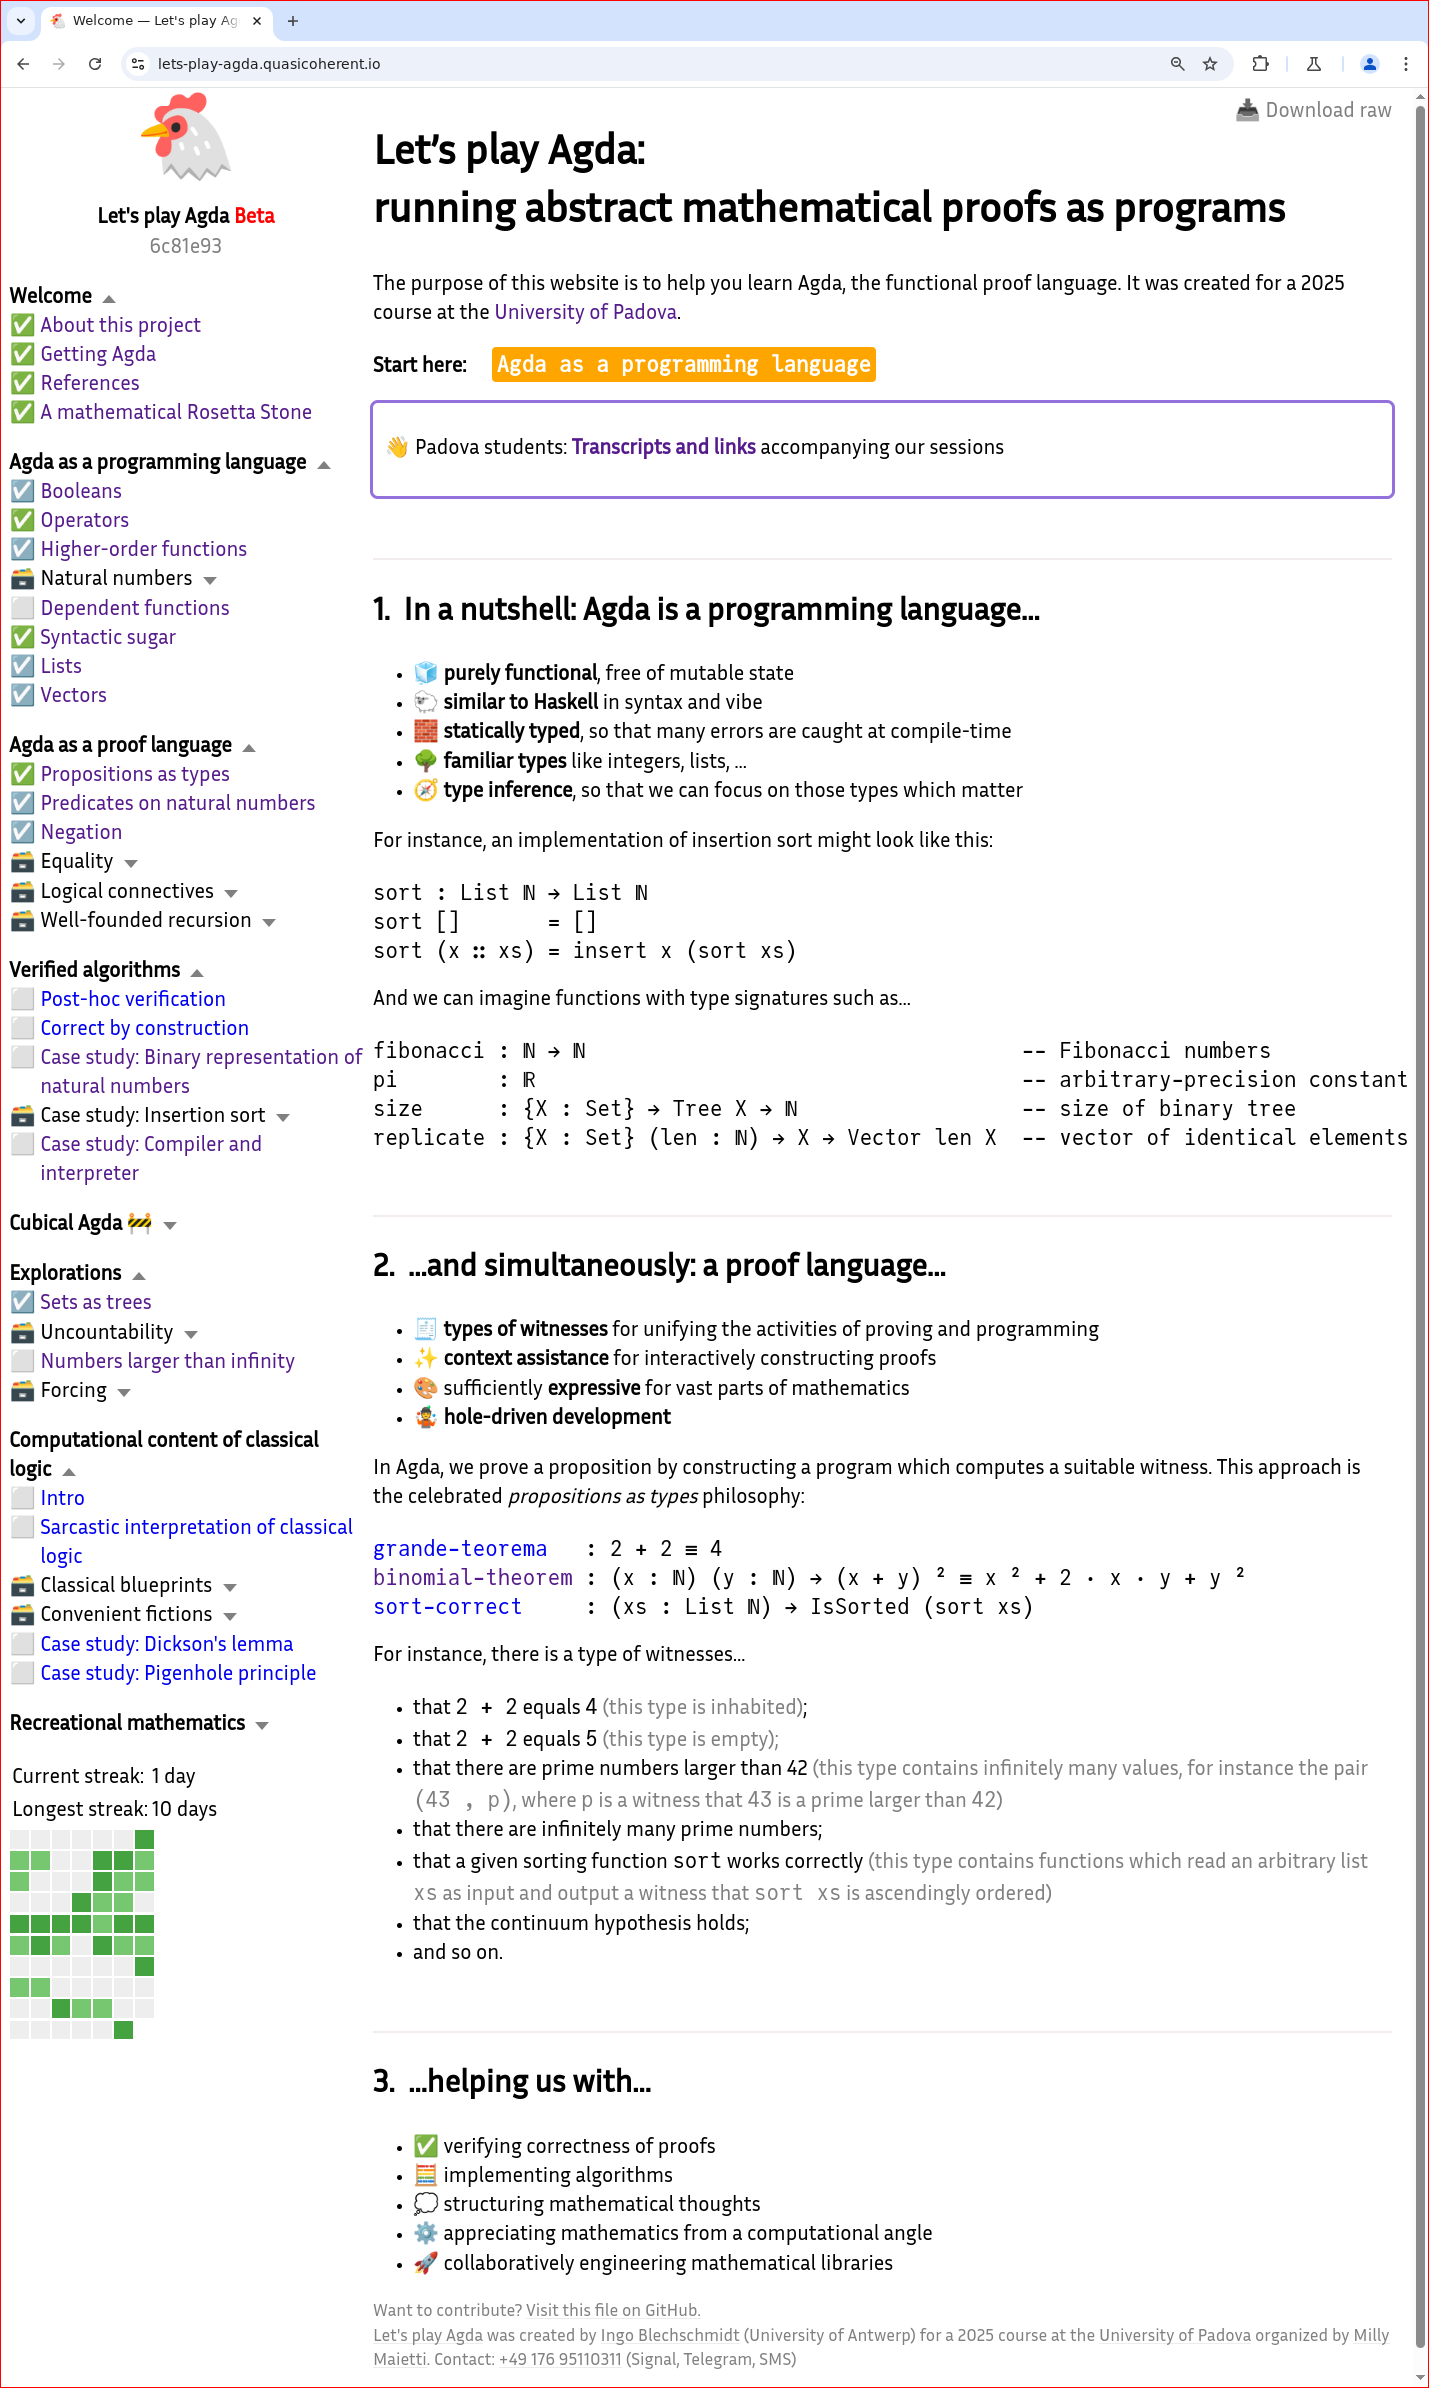
\includegraphics[width=0.95\textwidth]{lets-play-agda}
    \end{column}
    \begin{column}{0.5\textwidth}
      
\includegraphics[width=0.8\textwidth]{ai-2025}

      \vspace*{-1.5cm}\hspace*{2cm}
      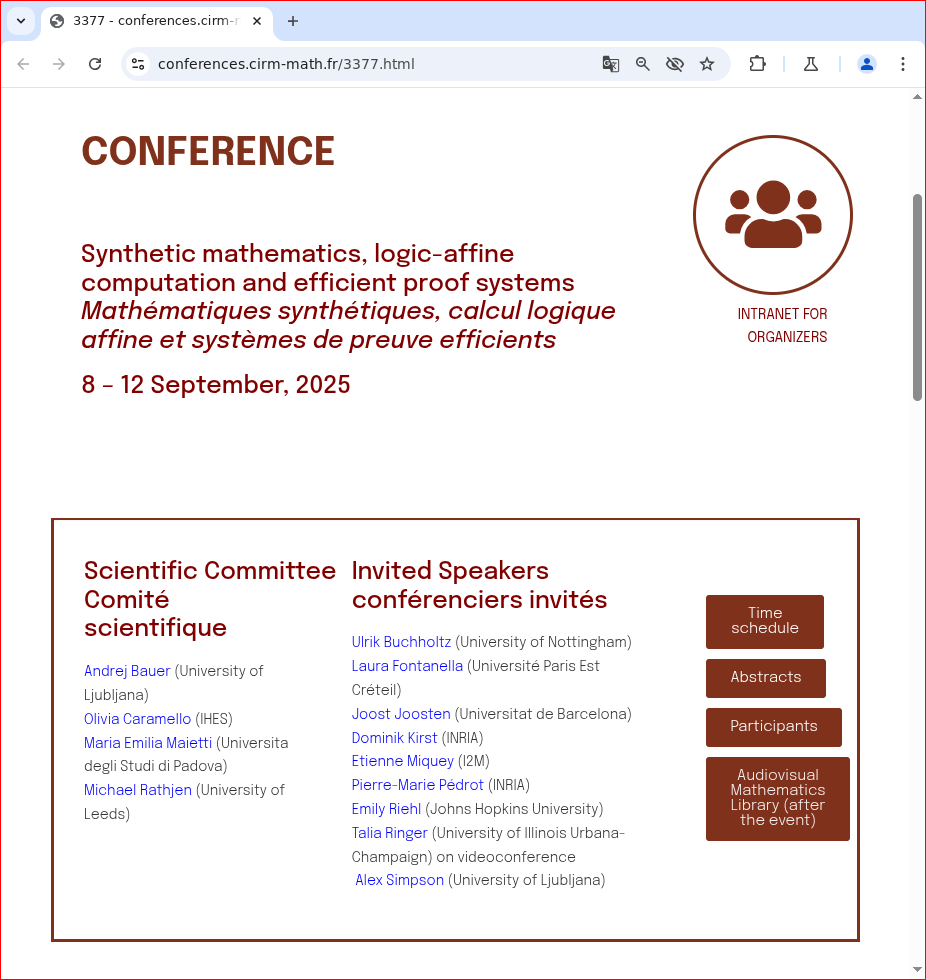
\includegraphics[width=0.8\textwidth]{cirm-2025}

      \vspace*{1cm}
    \end{column}
  \end{columns}
\end{frame}

\begin{frame}
  \emph{Backup slides.}
\end{frame}

\section{Basics of forcing}

\begin{frame}{Ingredients for forcing}
  \vspace*{-0.3em}
  To construct a forcing extension, we require:
  \begin{enumerate}
    \item a base universe~$V$
    \item a preorder~$L$ of \hil{forcing conditions} in~$V$\!,
    pictured as \hil{finite approximations}

    (\emph{convention:} $\tau \preccurlyeq \sigma$ means that~$\tau$ is a
    better finite approximation than~$\sigma$)
    \item a \hil{covering system} governing how finite approximations evolve to
    better ones

    (for each~$\sigma \in L$, a set~$\Cov(\sigma) \subseteq
    P({\downarrow}\sigma)$, with a simulation condition)
  \end{enumerate}
  In the forcing extension~$V^\nabla$, there will then be a \hil{generic filter} (ideal
  object).
  \pause

  \vspace*{-1em}
  \begin{columns}
    \begin{column}{0.49\textwidth}
      \small
      \begin{block}{For the generic surjection~$\NN \twoheadrightarrow X$}
        \justifying
        Use \hil{finite lists}~$\sigma \in X^*$ as forcing conditions,
        where $\tau \preccurlyeq \sigma$ iff~$\sigma$ is an initial segment of~$\tau$,
        and be prepared to grow~$\sigma$ to \ldots
        \footnotesize
        \begin{enumerate}
          \item[(a)] one of~$\{ \sigma x \,|\, x \in X \}$, to make~$\sigma$ more defined
          \item[(b)] one of~$\{ \sigma \tau \,|\, \tau \in X^*, a \in
          \sigma\tau \}$, for any~$a \in X$, to make~$\sigma$ more surjective
        \end{enumerate}
        \vspace*{-0.4em}
      \end{block}
    \end{column}
    \pause

    \begin{column}{0.45\textwidth}
      \small
      \begin{block}{For the generic prime ideal of a ring~$A$}
        \justifying
        Use \hil{f.g.\@ ideals} as forcing conditions, where $\bbb \preccurlyeq
        \aaa$ iff~$\bbb \supseteq \aaa$, and be prepared to grow~$\aaa$ to \ldots
        \footnotesize
        \begin{enumerate}
          \item[(a)] one of~$\emptyset$, if~$1 \in \aaa$, to make~$\aaa$ more proper
          \item[(b)] one of~$\{ \aaa+(x), \aaa+(y) \}$, if~$xy \in \aaa$, to
          make~$\aaa$ more prime
        \end{enumerate}
        \vspace*{-0.4em}
      \end{block}
    \end{column}
  \end{columns}
\end{frame}

{\usebackgroundtemplate{\begin{minipage}{\paperwidth}\vspace*{-1cm}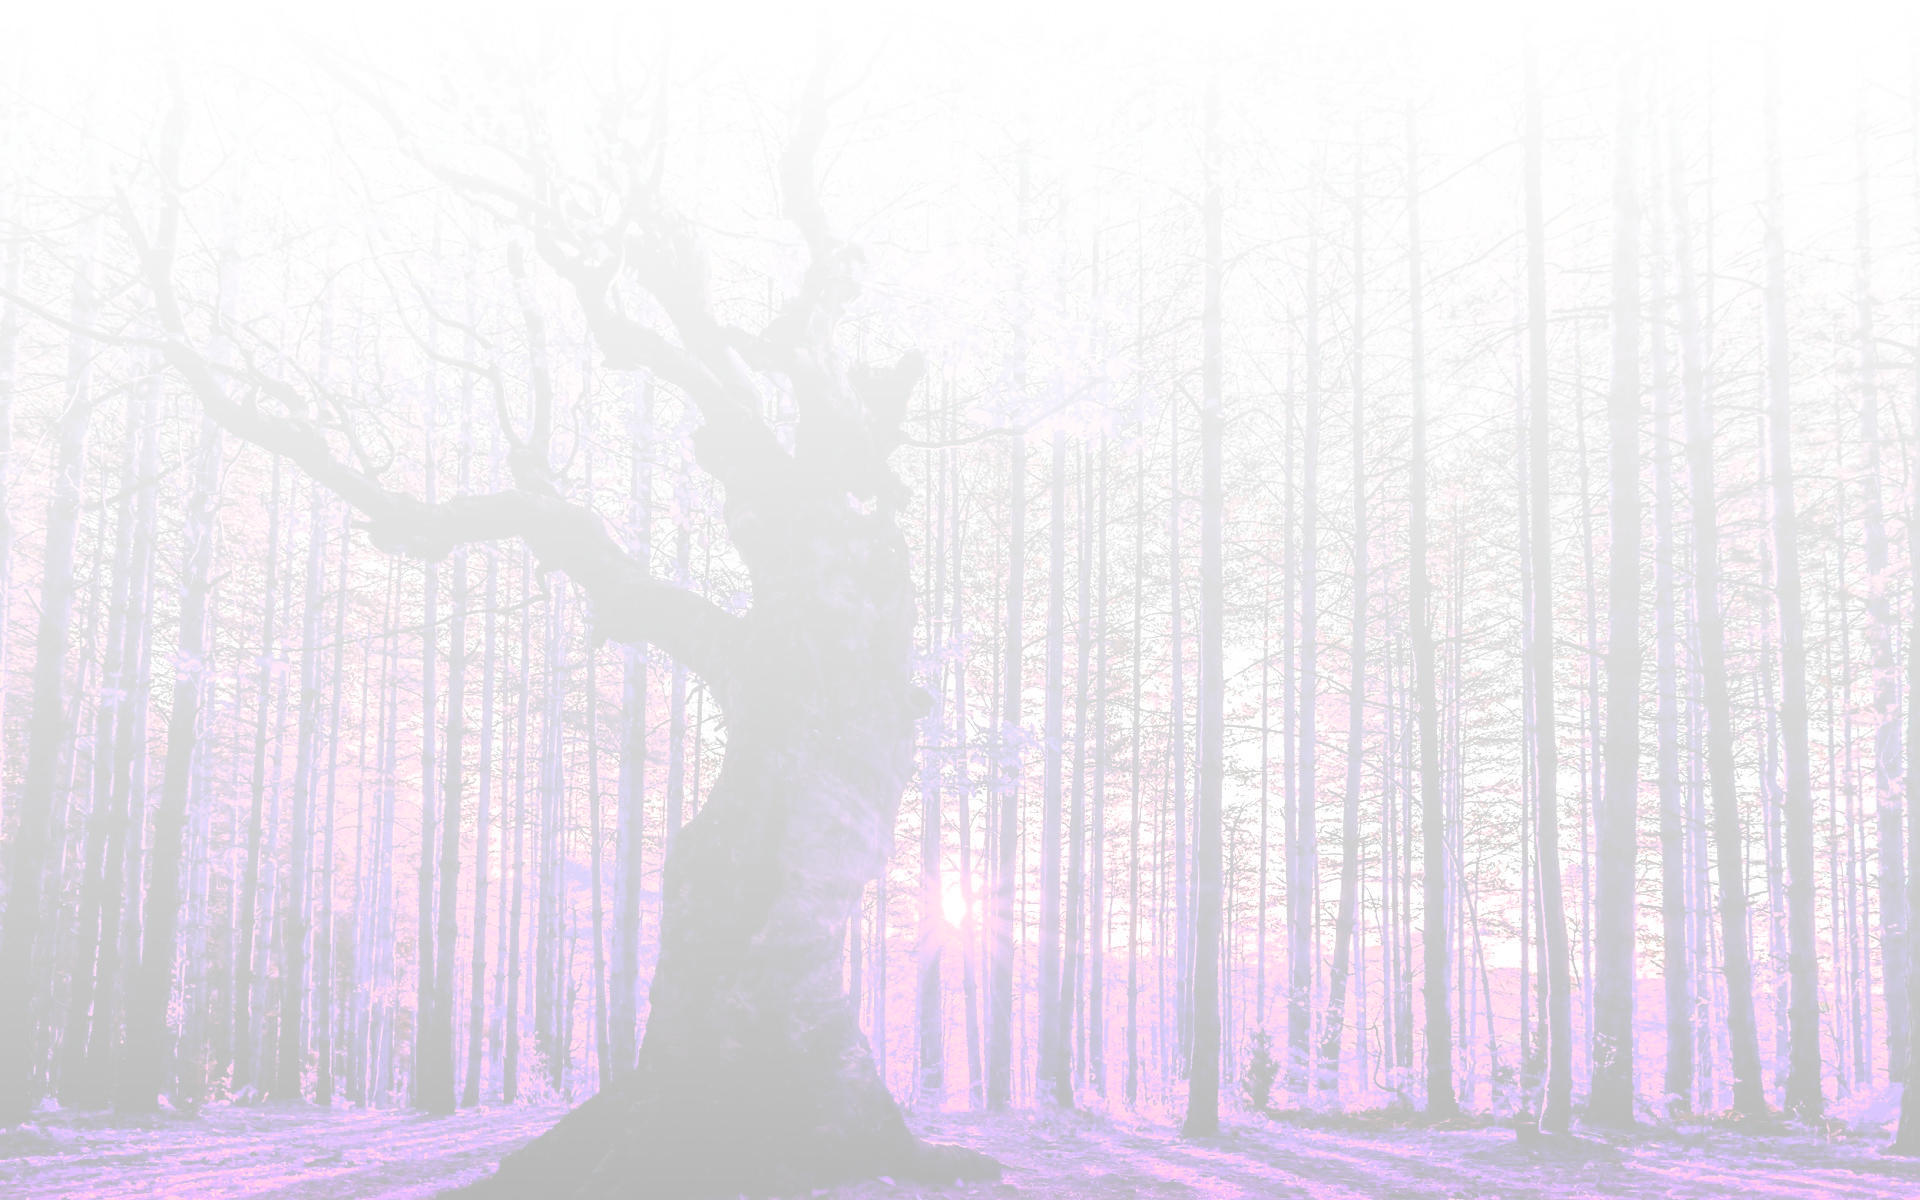
\includegraphics[width=\paperwidth]{forest-light-colored}\end{minipage}}
\begin{frame}{The eventually monad}
  Let~$L$ be a forcing notion.

  Let~$P$ be a monotone predicate on~$L$
  (if $\tau \preccurlyeq \sigma$, then $P\sigma \Rightarrow P\tau$). \\
  For instance, in the case~$L = X^*$:
  \begin{itemize}
    \item $\mathsf{Repeats}\, x_0\ldots x_{n-1} \defeqv \exists i\_ \exists j\_ i < j \wedge x_i = x_j$
    \item $\mathsf{Good}\, \,\,\,\,\,\,x_0\ldots x_{n-1} \defeqv \exists i\_ \exists j\_ i < j \wedge x_i \leq x_j$
    \quad (for some preorder~$\leq$ on~$X$)
  \end{itemize}
  \pause

  We then define~``\hil{$\nabla\,P\,\sigma$}'' (``$P$ bars~$\sigma$'') inductively by the following clauses:
  \begin{enumerate}
    \item If~$P\sigma$, then~$\nabla\,P\,\sigma$.
    \item If~$\nabla\,P\,\tau$ for all~$\tau \in R$, where~$R$ is some covering
    of~$\sigma$, then~$\nabla\,P\,\sigma$.
  \end{enumerate}
  So~$\nabla\,P\,\sigma$ expresses in a \hil{direct inductive fashion}:
  \[ \text{``No matter
  how~$\sigma$ evolves to a better approximation~$\tau$, eventually~$P\,\tau$
  will hold.''} \]

  \pause
  We use quantifier-like notation: ``$\nabla(\tau \preccurlyeq \sigma)\_
  P\tau$'' means ``$\nabla\,P\,\sigma$''.
\end{frame}}
% BOARD:
% - examples for P | σ
% - abuse of notation

\begin{frame}{Proof translations}
  \textbf{Thm.} Every~\textsc{iqc}-proof remains correct, with at most a
  polynomial increase in length, if throughout we
  replace
  \[\begin{array}{rcl@{\quad\text{where}\quad}rcl}
    \exists & \leadsto & \exists^\mathrm{cl},
    & \exists^\mathrm{cl} &\defeqv& \neg\neg\exists, \\
    \vee & \leadsto & \vee^\mathrm{cl},
    & \alpha \vee^\mathrm{cl} \beta &\defeqv& \neg\neg(\alpha \vee \beta), \\
    = & \leadsto & =^\mathrm{cl},
    & s =^\mathrm{cl} t &\defeqv& \neg\neg(s = t).
  \end{array} \]
  \pause

  \begin{columns}[c]
    \begin{column}{0.01\textwidth}
      
\includegraphics[height=2.4em]{sheafification-man-2}
    \end{column}
    \quad
    \begin{column}{0.9\textwidth}
      \hil{When we say:}\ \ some statement ``holds in~$V^{\neg\neg}$'', \\
      \makesamewidth[l]{\hil{When we say:}}{\hil{we mean:}}\ \ its translation holds in~$V$.
    \end{column}
  \end{columns}
  \bigskip

  Similarly for arbitrary forcing extensions~$V^\nabla$, ``just with~$\nabla$
  instead of~$\neg\neg$''.
  \bigskip

  \pause
  \textbf{Ex.} As~$\neg\neg(\varphi \vee \neg\varphi)$ is a theorem
  of~\textsc{iqc}, the law of excluded middle holds in~$V^{\neg\neg}$.
\end{frame}

\newcommand{\defeqvi}{\quad iff\quad}
\begin{frame}{The $\nabla$-translation}
  \small
  \only<1>{For bounded first-order formulas over the (large) first-order signature which has
  \begin{enumerate}
    \scriptsize
    \item one sort~$\underline{X}$ for each set~$X$ in the base universe,
    \\[-1.2em]
    \item one~$n$-ary function symbol~$\underline{f} : \underline{X_1} \times
    \cdots \times \underline{X_n} \to \underline{Y}$ for each map~$f : X_1 \times
    \cdots \times X_n \to Y$,
    \\[-1.2em]
    \item one~$n$-ary relation symbol~$\underline{R} \hookrightarrow
    \underline{X_1} \times \cdots \times \underline{X_n}$ for each relation~$R
    \subseteq X_1 \times \cdots \times X_n$, and
    \\[-1.2em]
    \item an additional unary relation symbol~$G \hookrightarrow \underline{L}$
    (for the \emph{generic filter} of~$L$),
  \end{enumerate}
  we recursively define:}
  \scriptsize
  \only<2->{\vspace*{-0.4em}}
  \begin{tabbing}
    \quad \= $\sigma \forces \forces \forall(x\?\underline{X})\_ \varphi$ \=
    \defeqvi $\textcolor{gray}{\forall(\tau \preccurlyeq \sigma)\_}\
    \forall(x_0 \in X)\_ \tau \forces \varphi[\underline{x_0}/x]$.\qquad\quad \=
    $\sigma \forces \exists(x\?\underline{X})\_ \varphi$
    \= $\sigma \forces \underline{R}(\underline{s_1},\ldots,\underline{s_n})$ \= \defeqvi $s = t$. \= \kill

    \> $\sigma \forces s = t$
    \> \defeqvi $\nabla \sigma\_ \llbracket s \rrbracket = \llbracket t \rrbracket$.
    \> $\sigma \forces \underline{R}(s_1,\ldots,s_n)$
    \> \defeqvi $\nabla\sigma\_ R(\llbracket s_1 \rrbracket,\ldots,\llbracket s_n \rrbracket)$. \\[0.3em]

    \> $\sigma \forces \varphi \Rightarrow \psi$
    \> \defeqvi $\textcolor{gray}{\forall(\tau \preccurlyeq \sigma)\_}\ (\tau \forces \varphi) \Rightarrow
    (\tau \forces \psi)$.
    \> $\sigma \forces G\tau$
    \> \defeqvi $\nabla\sigma\_ \sigma \preccurlyeq \llbracket\tau\rrbracket$. \\[0.3em]

    \> $\sigma \forces \top$ \> \defeqvi $\top$.
    \> $\sigma \forces \bot$ \> \defeqvi $\hil{$\nabla\sigma\_$}\ \bot$ \\[0.3em]

    \> $\sigma \forces \varphi \wedge \psi$
    \> \defeqvi $(\sigma \forces \varphi) \wedge (\sigma \forces \psi)$.
    \> $\sigma \forces \varphi \vee \psi$
    \> \defeqvi $\hil{$\nabla\sigma\_$}\ (\sigma \forces \varphi) \vee (\sigma \forces \psi)$. \\[0.3em]

    \> $\sigma \forces \forall(x\?\underline{X})\_ \varphi$
    \> \defeqvi $\textcolor{gray}{\forall(\tau \preccurlyeq \sigma)\_}\ \forall(x_0 \in X)\_ \tau \forces
    \varphi[\underline{x_0}/x]$.
    \> $\sigma \forces \exists(x\?\underline{X})\_ \varphi$
    \> \defeqvi $\hil{$\nabla\sigma\_$}\ \exists(x_0 \in X)\_ \sigma \forces \varphi[\underline{x_0}/x]$.
  \end{tabbing}
  \small
  \only<1>{Finally, we say that~$\varphi$ ``holds in~$V^\nabla$'' iff for all~$\sigma
  \in L$, $\sigma \forces \varphi$.}

  \footnotesize
  \begin{tabular}{@{}lp{0.27\textwidth}p{0.48\textwidth}@{}}
    \toprule
    forcing notion & statement about~$V^\nabla$ & external meaning \\
    \midrule
    surjection $\NN \twoheadrightarrow X$ &
    ``the gen.\@ surj.\@ is surjective'' &
    $\forall(\sigma{\in}X^*)\_ \forall(a{\in}X)\_ \nabla(\tau{\preccurlyeq}\sigma)\_ \exists(n{\in}\NN)\_ \tau[n] = a$. \\[0.4em]
    \pause

    map $\NN \to X$ &
    ``the gen.\@ sequence is good'' &
    $\mathsf{Good} \mid [\,]$. \\[0.4em]

    frame of opens &
    ``every complex number has a square root'' &
    For every open~$U \subseteq X$ and every cont.\@
    function $f : U \to \CC$, there is an open covering $U = \bigcup_i U_i$ such
    that for each index~$i$, there is a cont.\@ function $g : U_i \to \CC$
    such that~$g^2 = f$. \\[4.3em]

    big Zariski &
    ``$x \neq 0 \Rightarrow \text{$x$ inv.}$'' &
    If the only f.p.\@ $k$-algebra in which~$x = 0$ is the zero algebra,
    then~$x$ is invertible in~$k$.\\[1.5em]
    \pause

    little Zariski &
    ``every f.g. vector space does \emph{not~not} have a basis'' &
    \makesamewidth[l]{}{\phantom{x}}\hil{Grothendieck's generic freeness lemma}
  \end{tabular}
\end{frame}

\begin{frame}{Outlook}
  \begin{block}{Passing to and from extensions}
    \justifying\small
    \textbf{Thm.} Let~$\varphi$ be a \hil{bounded first-order formula} not
    mentioning~$G$. In each of the following situations, we have that
    $\varphi$ holds in~$V^\nabla$ iff~$\varphi$
    holds in $V$:

    \vspace*{-0.5em}
    \begin{enumerate}
      \item $L$ and all coverings are inhabited (proximality). \\[-1em]
      \item $L$ contains a top element, every covering of the
      top element is inhabited, and~$\varphi$ is a coherent implication
      (positivity).
    \end{enumerate}
    \vspace*{-0.8em}
  \end{block}

  \vspace*{-1.5em}
  \begin{columns}
    \begin{column}{0.46\textwidth}
      \begin{block}{The mystery of nongeometric sequents}
        \justifying
        The \hil{generic ideal} of a ring is maximal:
        \vspace*{-1em}
        \[ (x \in \aaa \Rightarrow 1 \in \aaa) \Longrightarrow 1 \in \aaa + (x). \]

        The \hil{generic ring} is a field:
        \vspace*{-0.7em}
        \[ (x = 0 \Rightarrow 1 = 0) \Longrightarrow (\exists y\_ xy = 1). \]
        \vspace*{-1.4em}
      \end{block}

    \end{column}

    \begin{column}{0.50\textwidth}
      \begin{block}{Traveling the multiverse \ldots}
        \textsc{lem} is a \hil{switch} and \hil{holds positively};
        being countable is a \hil{button}.
        \medskip

        Every instance of \textsc{dc} \hil{holds proximally}.
        \medskip

        A geometric implication is provable iff it holds \hil{everywhere}.
        \vspace*{-0.2em}
      \end{block}
      \vspace*{-0.3em}
      \hfill\footnotesize\ldots{} upwards, but always keeping ties to the
      base.{\ }
    \end{column}
  \end{columns}
\end{frame}

\begin{frame}{More on forcing notions}
  \small
  \textbf{Def.} A \hil{forcing notion} consists of
  a preorder~$L$ of \hil{forcing conditions}, and
  for every~$\sigma \in L$, a set~$\Cov(\sigma) \subseteq
  P({\downarrow}\sigma)$ of \hil{coverings} of~$\sigma$
  such that: If~$\tau \preccurlyeq \sigma$ and~$R \in \Cov(\sigma)$, there
  should be a covering~$S \in \Cov(\tau)$ such that~$S \subseteq
  {\downarrow}R$.
  \bigskip

  {\centering\footnotesize\begin{tabular}{llll}
    \toprule
    & preorder~$L$ & coverings of an element~$\sigma \in L$ & filters of~$L$ \\
    \midrule
    \normalnumber{1} & $X^*$ & $\{ \sigma x \,|\, x \in X \}$ & maps~$\NN \to X$ \\
    \normalnumber{2} & $X^*$ & $\{ \sigma x \,|\, x \in X \}$,\ \ $\{ \sigma\tau \,|\, \tau \in X^*, a \in \sigma\tau \}$ for each~$a \in X$ & surjections~$\NN \twoheadrightarrow X$ \\
    \normalnumber{3} & f.g. ideals & --- & ideals \\
    \normalnumber{4} & f.g. ideals & $\{ \sigma+(a), \sigma+(b) \}$ for each~$ab \in \sigma$,\ \ $\{\}$ if~$1 \in \sigma$ & prime ideals \\
    \normalnumber{5} & opens & $\mathcal{U}$ such that~$\sigma = \bigcup \mathcal{U}$ & points \\
    \normalnumber{6} & $\{\star\}$ & $\{ \star \,|\, \varphi \} \cup \{ \star \,|\, \neg\varphi \}$ &
    witnesses of~\textsc{lem}
    \\
    \bottomrule
  \end{tabular}\par}
  \bigskip

  \textbf{Def.} A \emph{filter} of a forcing notion~$(L,\mathrm{Cov})$
  is a subset~$F \subseteq L$ such that
  \vspace*{-0.4em}
  \begin{enumerate}
    \scriptsize
    \item $F$ is upward-closed: if~$\tau \preccurlyeq \sigma$ and if~$\tau \in F$, then~$\sigma \in F$; \\[-3.0em]
    \item $F$ is downward-directed: $F$ is inhabited, and if~$\alpha,\beta \in F$,
    then there is a common refinement~$\sigma \preccurlyeq \alpha,\beta$ such
    that~$\sigma \in F$; and \\[-2.0em]
    \item $F$ splits the covering system: if~$\sigma \in F$ and~$R \in
    \Cov(\sigma)$, then~$\tau \in F$ for some~$\tau \in R$.
  \end{enumerate}
\end{frame}

\backupend

\end{document}

0. A play in classical logic

1. Hilbert's program
   - basics about wqo's
   - subsequence lemma
   - Dickson
   - inductive reimagination
   - questions: where from? why work? how much stronger?

2. Where do our most cherished definitions come from?
   - a familiar business: enlarging mathematical structures
   - adjoining generic function, surjection, prime ideal, ...
   - observations:
     - well iff generic sequence is good iff everywhere, every sequence is good
       (in particular, every multivalued and every up-to-¬¬-defined sequence is good)
     - wellfounded iff for the generic decreasing sequence, ⊥ iff ...
   - fun facts about generic gadgets

3. Modal language for harnessing the multiverse
   - definition
   - examples
   - implicational wellness
   - dialogue

4. Implementation
   - idea: realize generic gadget as some kind of limit of approximations from
     the base
   - reinterpret, in a mechanic fashion, assertions about generic objects as
     assertions about approximations
     - ex.: "the generic function is defined on input n" as "no matter how the
       empty list evolves over a time to a better approximation xs, eventually
       xs will have length at least succ n"
   - crucially, this interpretation is sound with respect to intuitionistic
     reasoning

5. Let's play Agda, CIRM, AI

---

Towards topological type theory for decrypting transfinite methods in classical mathematics

In constructive mathematics, an ongoing challenge is to extracting
computational content from infinitary arguments in classical
mathematics—especially those that yield concrete results via abstract tools
such as minimal bad sequences or maximal ideals. Today, a wide range of such
techniques exists, constituting a late partial fulfillment of Hilbert's
program.

This talk presents work in progress on porting the modal operators "everywhere"
and "somewhere", as developed in set theory by Joel David Hamkins, Victoria
Gitman and their collaborators, into type theory. This modal enrichment
provides a uniform language for expressing several established
constructivization techniques, and is at the core of a relatively recent new
technique that offers insights on the origins of some of our most cherished
inductive definitions. These developments are closely connected to recent
advances in type-theoretic presheaf and sheaf models, dialogue
continuity, synthetic algebraic geometry and well-quasi-order theory.

---

Which functions are we excluding when we form the type of all functions between
two types? Does every field have an algebraic closure?

Inspired by the modal approach to the set-theoretic multiverse of Joel David
Hamkins, Victoria Gitman and their collaborators, we aim to introduce the modal
operators "everywhere" and "somewhere" to homotopy type theory, proposing a
multiversal perspective on these motivating questions.

---

Well quasi-orders are a combinatorial notion with featureful applications in
graph theory, termination checking, commutative algebra and other subjects.
However, their classical definition, though concise and elegant, poses
significant challenges in constructive mathematics and frameworks that lack
function sets. In response, several constructive substitutes have been
developed, most recently an implicational definition by Stefano Berardi,
Gabriele Buriola and Peter Schuster. In this talk, we investigate how a modal
approach can reinterpret classical proofs involving transfinite methods as
blueprints for constructive proofs grounded in these alternatives, thereby
combining the best of both worlds: Short and abstract proofs, but with
constructive content. We also indicate how the modal approach allows us to
compare the implicational definition with an earlier inductive one.

---

Combinatorics and commutative algebra abound with situations where we prove
quite concrete results by quite abstract transfinite methods, such as minimal
bad sequences or maximal ideals. Amazingly, such infinitary arguments can often
be understood as blueprints for quite explicit computations—as called for by
Hilbert’s programme. In this talk, we will travel the modal toposophic
multiverse to facilitate this kind of mining abstract proofs for refined
quantitative results. We will use a celebrated theorem from order theory about
sequences N→N that everybody can relate with as a running example.

---

Where do some of our most cherished inductive definitions come from? Which
functions are we excluding when we form the type of all functions between two
types? Does every field have an algebraic closure?

Inspired by the modal approach to the set-theoretic multiverse of Joel David
Hamkins, Victoria Gitman and their collaborators, we aim to introduce the modal
operators "everywhere" and "somewhere" to homotopy type theory, proposing a
multiversal perspective on these motivating questions.

Unlike the set-theoretic role model, we focus less on exploring the range of
foundational possibility and more on concrete applications in constructive
mathematics, with the goal of porting results of classical mathematics to
homotopy type theory. It will turn out that every field has an algebraic
closure somewhere; that a transitive relation is well-founded iff nowhere there
is an infinite descending chain; and that somewhere, the law of excluded middle
holds.

This is ongoing joint work with Alexander Oldenziel and connected to the recent
advances with type-theoretic presheaf models and sheaf models.
